\chapter{Relativistic formulations}
\label{ch:Relativity}


A detailed description of relativistic field theory can be found in~\cite{LandauLip}. Here, we remind the reader about some useful relations and definitions.


\section{A few definitions}


\begin{itemize}
\item[$\bullet$] \textbf{Four-vector:}(\textbf{4-vector}): $R$ et $R'$ designate two Galilean referentials, a four-vector $v_{R}$ is by definition a vector which expression from $R$ to $R'$ is given by the Lorenz transformation  $v_{R'} = L_{\mu}^{\nu} v_{R}$. 
\item[$\bullet$] \textbf{Four-scalar}(\textbf{4-scalar}): Scalar invariant from $R$ to $R'$. Example of 4-scalars: electric charge, phase ($\omega t-kr$) of electromagnetic radiation, proper time.
\item[$\bullet$]\textbf{Proper time $\tau$:} Time intrinsically linked to a particle in motion. If $t$ is the time in $R$ we have $dt = \gamma d\tau$, with $\gamma = (1-\frac{v(t)^2}{c^2})^{-1/2}$. An expression of $\tau(t)$ is obtain with the equation of motion. However, since $ \gamma > 0$, $\tau$ is necessarily strictly increasing with $t$, which means we can invert the expression to express $t(\tau)$. \\
\end{itemize}

\vspace{0.1in}

\noindent Examples of 4-vectors:\\

\begin{center}
\begin{tabular}{p{5cm}cc}
4-vector & Einstein notation & Normal notation \\
\g{4-position} & $x^{\mu}(t)$ & $(ct,\g{r}(t))$\\
\g{4-current} & $j^i = \rho \frac{dx^i}{dt}$ &$ (\rho c , \rho \g{v})$ \\
\g{4-current} & $j^i = \rho \frac{dx^i}{dt}$& $(\rho c , \rho \g{v})$ \\
\g{4-wavevector} & $k^{i} $& $ (\frac{\omega}{c} ,\g{k})$\\
\g{4-vector potential} & $\mathcal{A}^{\mu}(x^{\mu}) $& $  (V(x^{\mu})/c ,\vec A(x^{\mu}))$\\
\end{tabular}
\end{center}





\noindent The \textbf{4-velocity}: obtained by the derivation of the 4-position relative to proper time. This way, we simply have:

$$
u^{\mu} = \frac{d x^{\mu}(t(\tau))}{d\tau} =  (\frac{dt(\tau)}{d\tau} c , \frac{d\g{r} (t(\tau))}{d\tau}) = (\gamma c , \gamma \frac{d\g{r}(t)}{dt})
$$

\noindent Note that since the 4-position is a 4-vector:
$$
x^{\mu}(t)' = \mathcal{L}^{\mu}_{\nu}(t)x^{\nu}(t)
$$
\noindent and therefore, the 4-velocity is also a 4-vector:
$$
u'^{\mu} = \gamma \frac{dx'^{\mu}}{dt} = \gamma \frac{ d (\mathcal{L}^{\mu}_{\nu}(t)x^{\nu}(t) )}{dt} = = \gamma \frac{ d (\mathcal{L}^{\mu}_{\nu}(t)}{dt} x^{\nu}(t)  +  \gamma \mathcal{L}^{\mu}_{\nu}(t) \frac{ d (x^{\nu}(t) )}{dt} = \mathcal{L}^{\mu}_{\nu} u^{\nu}
$$

\noindent This demonstration is only valid for a Galilean referential  (ie $ \frac{d (\mathcal{L}^{\mu}_{\nu}(t)}{dt} = 0$ ). 
One should be careful that "$\gamma $" has two implicit definitions: 
First, the most common, is used in the definition of the proper time, where $v$ denotes the particle velocity. 
Second,  the analytical expression if the same , but $\g{v}$ now corresponds to the (constant !) velocity of the Galilean referential used in the definition of $\mathcal{L}^{\mu}_{\nu}$.

\noindent The \textbf{4-acceleration} is obtained by derivation of the 4-velocity relative to proper time: 
$$
\Gamma^{\mu} (t) = \frac{d u^{\mu}}{d\tau} = (c\gamma \frac{d\gamma}{dt},\gamma \frac{d\gamma}{dt}\vec v + \gamma^2 \vec a)
$$


\section{Relativistic equation of motion for a charged particle}


%\begin{equation}
%\lambda >> \frac{e^2}{mc} \approx 4\times 10^{-25}
%\end{equation}

The derivation of the equation is properly done in~\cite{LandauLip} using a principle of least action applied on a charge $q$ of mass $m$ in an electromagnetic field. In many publications~\cite{kibble1966mutual,schmidt1973relativistic}, it is given using tensorial Einstein notation:

\begin{equation}
\frac{du^i}{d\tau} = \frac{q}{mc}(\partial_{x^i}A^k - \partial_{x^k}A^i)u_k 
\end{equation}

\noindent Which is equivalent to:

\begin{subequations}
\label{relativisticMotionEq}
\begin{align}[left = \empheqlbrace\,]
&\frac{d}{dt}[\gamma \g{v} + \frac{q}{m}\g{A}] = \frac{q}{m}(\g{v}\nabla)\g{A} + \frac{q}{m}\g{v}\times (\nabla \times \g{A}) + q\nabla \phi \label{relativisticMotionEq-1} \\
&\frac{dE_{kin}}{dt} = \frac{d}{dt}\left( \gamma mc^2 \right) = q\g{E}\g{v} \label{relativisticMotionEq-2}
\end{align}
\end{subequations}

\noindent With the relation $(\g{v}.\nabla)\g{A} + \g{v}\times (\nabla \times \g{A}) = (\g{v}\times \nabla)\times \g{A} + (\nabla.\g{A})\g{v}$, Eq~\ref{relativisticMotionEq-1} can also be transformed into:


\begin{subequations}
\label{relativisticMotion3equation}
\begin{align}[left = \empheqlbrace\,]
&\frac{d}{dt}[\gamma v_x + \frac{q}{m}A_x] =\frac{q}{m_e}\g{v}\partial_x \g{A} + q\partial_x\phi \\
&\frac{d}{dt}[\gamma v_y + \frac{q}{m}A_y] = \frac{q}{m_e}\g{v}\partial_y \g{A}+ q\partial_y\phi \\
&\frac{d}{dt}[\gamma v_z + \frac{q}{m}A_z] = \frac{q}{m_e}\g{v}\partial_z \g{A}+ q\partial_z\phi
\end{align}
\end{subequations}

\noindent If on the contrary we develop the left-hand side of Eq~\ref{relativisticMotionEq-1}, and use the relation $\frac{d\g{A}}{dt} = \partial_t\g{A} + (\g{v}\nabla)\g{A}$, we find the well-known equation:

\begin{equation}
\frac{d}{dt}[\gamma \g{v} ]= \frac{q}{m}\g{E}+ \frac{q}{m}\g{v}\times \g{B}
\end{equation}


\section{Gauge invariance}

The 4-vector $A_k = (\phi/c,A_x,A_y,A_z)$ contains all information about the electromagnetic fields $(E,B)$ at play in the equation of motion. Choosing the gauge consists in imposing a condition on $A_k$ which has no impact on the equation of motion, but could simplify the analytical resolution of the equation.
The $(E,B)$ fields are expressed by: 

\begin{equation}
  \left\{
      \begin{aligned}
     &  \g{B}= \nabla \times (\g{A}+ \nabla f(r,t)) = \nabla \times \g{A}\\
     & \g{E}= - \nabla \left( \phi -\partial_tf(r,t)\right) - \partial_t (\g{A}+ \nabla f(r,t)) =- \nabla \phi - \partial_t \g{A} \\
      \end{aligned}
    \right.
\end{equation}

\noindent Therefore, one can choose an additional scalar equation verified by the components $(\phi/c,A_x,A_y,A_z)$, which is equivalent to choosing a function $f$. For example if $F$ is a linear 
partial differential equation verified by $A_k$ (i.e. $F(A_k) = 0$), the corresponding gauge will be a solution of the differential system:

\begin{equation}
F((\partial_t f, \nabla f)) =- F(A_k) 
\end{equation}

\begin{center}
\begin{tabular}{p{5cm}c}
Lorenz Gauge& $\nabla \g{A}+ \frac{1}{c^2}\partial_{t}\phi = 0$\\
Coulomb Gauge & $\nabla \g{A} = 0$ \\
\end{tabular}
\end{center}




%
%
%
%
%
%\subsection{Lab frame to Bourdier frame}
%
%
%\begin{figure}[H]
%\centering
%\fbox{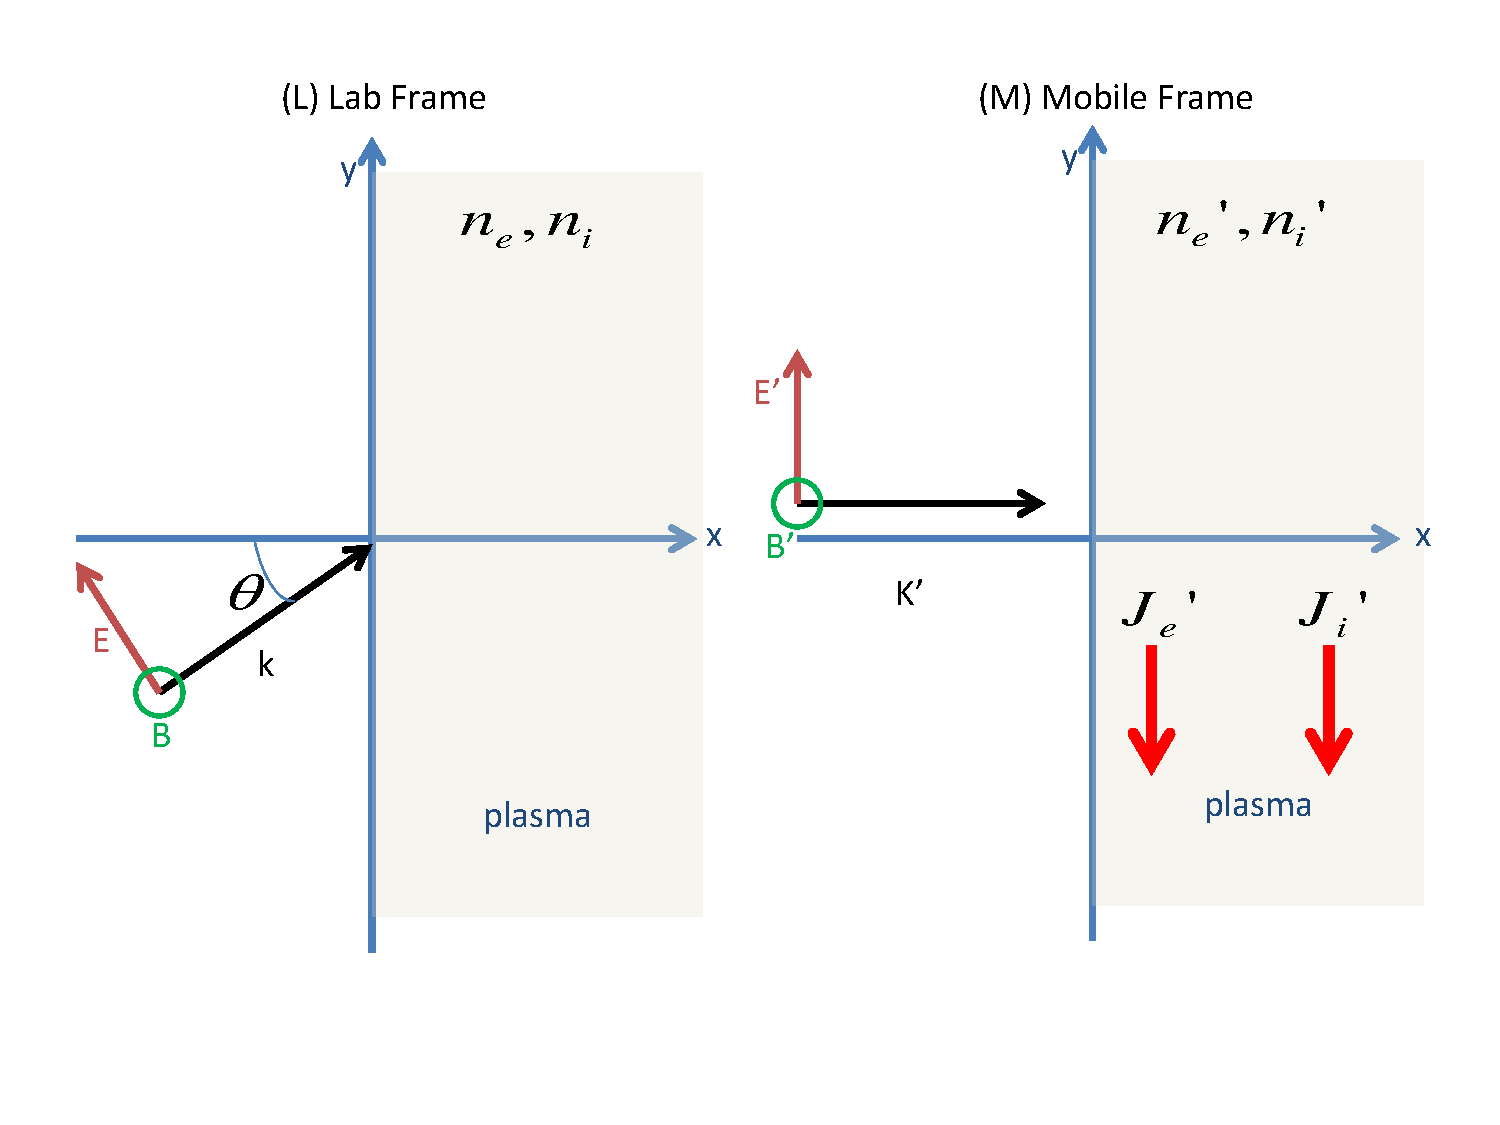
\includegraphics[width =0.9\textwidth]{../Annexe/images/1DBoostedFrame.pdf}}\\
%\caption{Transformation from lab frame referential (R) to mobile frame referencial (M), also called Bourdier referencial. The (M) velocity defined in (L) is equal to $\vec{v} = csin(\theta)\vec{u}_y$ We impose to the incident wave to be plane and to verify in the referencial L: $\vec{k} = (\frac{\omega}{c}cos(\theta),\frac{\omega}{c}sin(\theta),0)$}
%\end{figure}
%
%\noindent In relativity, all fourvectors $X \in \mathbb{R}^4$ defined in referencial $(R)$ will be retrieve in $(M)$using a lonrenzian transform:
%$$
%X' =\mathcal{L}X
%$$
%\[
%\mathcal{L}=
%  \begin{bmatrix}
%    \gamma & 0 & -\beta\gamma & 0 \\
%    0 & 1 & 0 & 0 \\
%    -\beta\gamma & 0 & \gamma & 0 \\ 
%     0 & 0 & 0 & 1\\      \end{bmatrix}
%\]
%
%\noindent Where $\beta = \frac{v}{c} = sin(\theta)$ and $\gamma = \frac{1}{\sqrt{1-\beta^2}}$
%
%
%
%We simply derivate the corresponding electromagnetic field by taking into account the spacial tranformation of the space coordinate such that for the incident field:
%
%\begin{equation}
%  \left\{
%      \begin{aligned}
%       & E'_x = \gamma (E_x + v B_z) \\
%       & E'_y = E_y  \\
%       & E_z' = \gamma (E_z - v B_x) \\
%       & B_x' =\gamma (B_x -\frac{v}{c^2}E_z)  \\
%       & B_y' =B_y\\
%       & B_z' = \gamma (B_y + \frac{v}{c^2}E_x) \\
%      \end{aligned}
%    \right.
%\end{equation}


%\begin{equation}
%  \left\{
%      \begin{aligned}
%       & E'_x = \gamma (E_x + v B_z) = \frac{1}{cos(\theta)}(-Esin(\theta) + Esin(\theta)(cos(\theta)^2+sin(\theta)^2))=0 \\
%       & E'_y = E_y = Ecos(\theta)  \\
%       & E_z' = \gamma (E_z - v B_x) = 0\\
%       & B_x' =\gamma (B_x -\frac{v}{c^2}E_z) = 0 \\
%       & B_y' =B_y = 0\\
%       & B_z' = \gamma (B_y + \frac{v}{c^2}E_x) = \frac{1}{cos(\theta)}\frac{sin(\theta)}{c}(-Esin(\theta)) \\
%      \end{aligned}
%    \right.
%\end{equation}
%
%We see here that the result of the transformed field fits where the graphical representation given in Fig ? where the incident electromagnetic field is along $z$ and the electric field alon $y$.
%An important remark is that looking at the critical density in $M$, we have using the quadrivector relations:
%
%$$
%n_c' = \frac{(\omega_0')^2 e^2}{m_e\epsilon_0} = \frac{(\omega_0)^2cos(\theta)^2 e^2}{m_e\epsilon_0} = n_c cos(\theta)^2
%$$
%$$
%\frac{n'}{n_c'} = \frac{n/cos(\theta)}{n_c cos(\theta)^2} = \frac{1}{cos(\theta)^3}\frac{n}{n_c} 
%$$
%
%







